\chapter{Verification and testing}
\label{cha:testing}

This chapter presents the evaluation of DRI service which design and implementation
was described in the previous chapters. It starts with the description of a~test case
study that is used for this purpose. It aims to cover the crucial service functionalities. Then, a~service
test environment is discussed. In order to ease evaluation process a~notification service
mock has been created. Finally, in the following sections, the subsequent service requirements
are evaluated.


\section{Case study}
\label{case-study}
As a~case study for DRI evaluation we designed a~test scenario consisting of multiple
data manipulation steps within VPH-Share project. Thanks to administration rights to the
data stored on Openstack instance we were able to manually simulate data corruption and
unavailability issues. The test case consists of the following steps:

\begin{enumerate}
\item creating a~dataset and uploading initial archive data through VPH-Share federated cloud
storage access layer,
\item tagging newly created dataset as managed,
\item waiting for success notification (no errors) about previous step,
\item invoking on-request validation of the dataset,
\item waiting for successful dataset validation,
\item manuallly modifying dataset content,
\label{manual-modification}
\item invoking on-request validation for the second time,
\item waiting for integrity error -- data corruption,
\item manually erasing file from the dataset,
\item invoking on-request validation for the third time,
\item waiting for integrity error -- data unavailable. 
\end{enumerate}

In step \ref{manual-modification} the content of the dataset
is modified in two different ways -- every byte of the file is changed and only a~fraction of
the file is changed. Corruption detection always succeds in the first case, while the second
allows false positives to occur when using probability-based validation algorithm.\\

This scenario represents a~relatively easy test case. However, it is an excellent candidate for
automation in form of an integration test that runs during every new build of the component.
To automate it, we either need an integration test environment or such environment has to be
mocked at runtime. The extended description of each step with associated commands and actions
to be perfomed is presented in appendixes. 

\section{Deployment environment and configuration}

In order to evaluate DRI, the service was deployed in the production environment
of VPH-Share project. During the prototype phase, a~dedicated virtual machine running Linux
server with Apache Tomcat is used instead of Atomic Service instance. The deployment
of DRI comes down to uploading a~web application archive (WAR) to Tomcat server
instance. DRI at the time of writing this thesis provides REST interface (described
in detail in section \ref{dri-interface}) at \url{http://vph.cyfronet.pl:18080/driservice/}.
For testing purposes DRI was provided with two cloud storage providers, Amazon S3 account
and private instance of Openstack Swift infrastructure.\\

DRI periodical validation period was set to $30 min$. The validation algorithm parameters --
$k$ and $n$ -- were set to $10$ and $100$ respectively. This means that each file is divided
into $100$ blocks of equal size. The checksum of every block is stored in metadata registry
upon tagging file as managed. During the validation phase, only $10$ randomly selected blocks
(roughly $10 \%$ of the file size) are retrieved, their checksums computed and compared
with the original values. Such configuration ensures error detection rate on relatively low
level of probability, $10 \%$ for small size modification $e$ (where $e \ll |F|$). However, it is
proportional to the size of the modification when $e \sim |F|$ (see section \ref{algorithm-analysis}).


\section{Notification Service}
\label{notification-service}
At the time of writing this thesis, VPH-Share Cloud Platform still lacks usable notification service
mechanism. In order to enable DRI evaluation we created a~simple web page which mocks
notification service functionalities -- see figure \ref{fig:notification-service}. Its intent
is to display basic information about operations perfomed by DRI service. It is organized in
tabular view of notifications. A~notification is represented by one row and is always associated
with operation performed on single dataset. Each row consists of the following information:

\begin{enumerate}
\item \textbf{dataset name},
\item \textbf{notification status} -- a~short message informing whether operation succeded or failed,
\item \textbf{execution time} -- the time it took to perform the operation in seconds,
\item \textbf{time scheduled} -- the time when the operation started.
\end{enumerate}

\begin{figure}[h!]
	\centering
	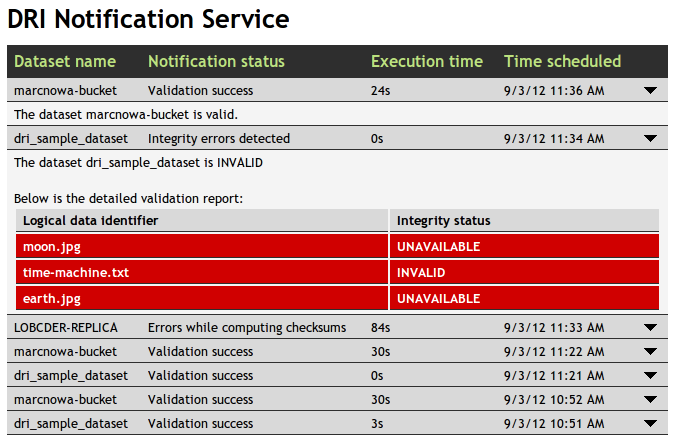
\includegraphics[width=\textwidth]{images/notification-service.png}
	\caption{Notification service mock overview -- it was created to evaluate DRI
	functional requirements. Notifications are organized in tabular view with
	basic information about the operation perfomed on a~single dataset. The details
	of data integrity errors -- whether containing file is invalid or unavailable --
	are presented after expanding each row.}
	\label{fig:notification-service}
\end{figure}

It is available at \url{http://vph.cyfronet.pl:18080/driservice/notification.jsp}.\\

Additional notification details are available for failed operation when it is
expanded. It can be seen which files within the given dataset caused problems --
either they are invalid or unavailable. For instance, the expanded 
\textit{dri\_sample\_dataset} notification shows that two files are unavailable
-- \textit{earth.jpg} and \textit{moon.jpg} -- and the \textit{time-machine.txt}
is corrupted.

\section{Functional requirements evaluation}
A key aspect of the DRI service is to meet its requirements within Cloud
Platform, which were listed in section \ref{requirements}. In the prototype
phase, we focus on data validation. As project continues, data
replication mechanisms will be developed within DRI service. As previous
chapters shown, we designed and implemented a service which enables periodic
and on-request data validation and notifies about any integrity or availability
errors. It can be used according to the REST interface described in chapter
\ref{cha:architecture}.

\subsection{Evaluation of periodic and on-request data validation}
The evaluation of DRI data validation mechanism is based on the test scenario described
in section \ref{case-study}. It was performed on DRI instance deployed in production
environment of VPH-Share project.




\section{Conclusions and results}
